\documentclass[18pt]{article}


\usepackage{graphicx}
\usepackage{polyglossia}
\usepackage{amsmath}
\usepackage{fontspec}
\setmainlanguage{greek}
\setotherlanguage{english}

\newfontfamily\greekfont{DejaVu Serif}
\setmainfont{DejaVu Serif}

\title{\Huge 2ndProject\_4713}
\author{\Large ΝΙΚΟΛΑΟΣ ΛΙΛΕΣ AEM: 4713}
\date{2025 - 2026}

\begin{document}
\maketitle

\newpage
\section*{Ασκηση 5: Προσέγγιση της συνάρτησης $\sin(x)$}

\vspace{0.5cm}
Στην 5η άσκηση σκοπός μας είναι \textbf{να προσεγγίσουμε την $sin(x)$ στο πεδίο [-π,π]}. Αρχικά επιλέγω \textbf{10 ισαπέχοντα σημεία} στο διαστημα και βρισκω τις \textbf{τιμες του ημιτόνου} στα σημεία αυτά.

Στη συνέχεια υλοποιώ 3 συναρτήσεις για τις 3 μεθόδους προσέγγισης του ημιτόνου\textbf{((α)Με πολυωνιμική, (β) Με splines, (γ) Με τη μέθοδο ελάχιστων τετραγώνων)} που μου ζητάει η εκφώνηση. Η υλοποίηση αυτή γίνετε στην γλώσσα προγραμματισμού \textbf{Python}.

\vspace{0.2cm}
\section*{(α) Πολυωνυμική προσέγγιση - Lagrange}
Με τη \textbf{μέθοδο Lagrange} κατασκευάζεται ενα πολυωνυμο που \textbf{περνάει απο τα 10 σημεία} που βρήκαμε προηγουμένως. Στον κώδικα που έγραψα, για κάθε τιμή του x που θέλω να υπολογίσω, \textbf{δημιουργώ τα πολυώνυμα με το γινόμενο των ώρων$(x - x_j)/(x_i - x_j)$} και έπειτα \textbf{αθροίζονται με τις αντίστοιχες τιμες της $sin(x)$}. \textbf{Η τελική τιμή} που επιστρέφετε (το p) \textbf{ειναι η προσέγγιση του ημιτόνου} στο συγκεκριμένο σημείο.


\vspace{0.2cm}
\section*{(β) Splines}
Στη \textbf{μέθοδο των splines} τη σημέια του ημιτόνου αρχικα\textbf{ πρέπει να ταξινομηθούν} και αυτο γίνετε με τη βοήθεια της συνάρτησης argsort. Για κάθε τιμή του x που θέλω να βρω, το προγραμμά μου βρίσκει \textbf{το διάστημα ανάμεσα σε 2 σημεία στο οποίο ανήκει}. Επειτα\textbf{ υπολογίζεται ένας συντελεστής που δείχνει τη θέση του x}και με βάση αυτόν\textbf{ γινεται γραμμική παρεμβολή ανάμεσα στα 2 σημεία}. Η τιμή που προκύπτει και επιστρέφετε ειναι η προσέγγιση του $\sin(x)$.


\vspace{0.2cm}
\section*{(γ) Ελαχίστων Τετραγώνων}
Στη μέθοδο αυτή προσεγγίζουμε την $\sin(x)$ με ενα \textbf{πολυωνυμο μικρού βαθμού}. Στον κώδικα αρχικά \textbf{δημιουργω εναν πίνακα με τις τιμές των δυνάμεων του x για τα 10 σημεία.} Επειτά, υπολογίζονται οι \textbf{συντελεστές του πολυωνυμου λύνοντας το αντίστοιχο σύστημα εξισωσεων}. Τελος, το πολυωνυμο αυτο υπολογίζεται σε κάθε τιμή του x και ετσι παιρνουμε την προσεγγιστικη τιμη του ημιτόνου.


\section*{Συγκρισή ακρίβειας μεθόδων}

\vspace{0.2cm}
Για τη συγκριση ακριβειας, στο πρόγραμμα \textbf{δημιουργουνται 200 ισαπέχοντα σημεία στο διάστημα [-π, π]} και σε κάθε σημείο υπολογίζω την πραγματική τιμη του ημιτόνου και την προσεγγιστική τιμη για την κάθε μέθοδο. Επειτά δημιουργώ ενα γράφημα για να δείξω πόσο καλα η κάθε μέθοδος προσεγγίσει το ημίτονο.
\vspace{0.2cm}

\begin{center}
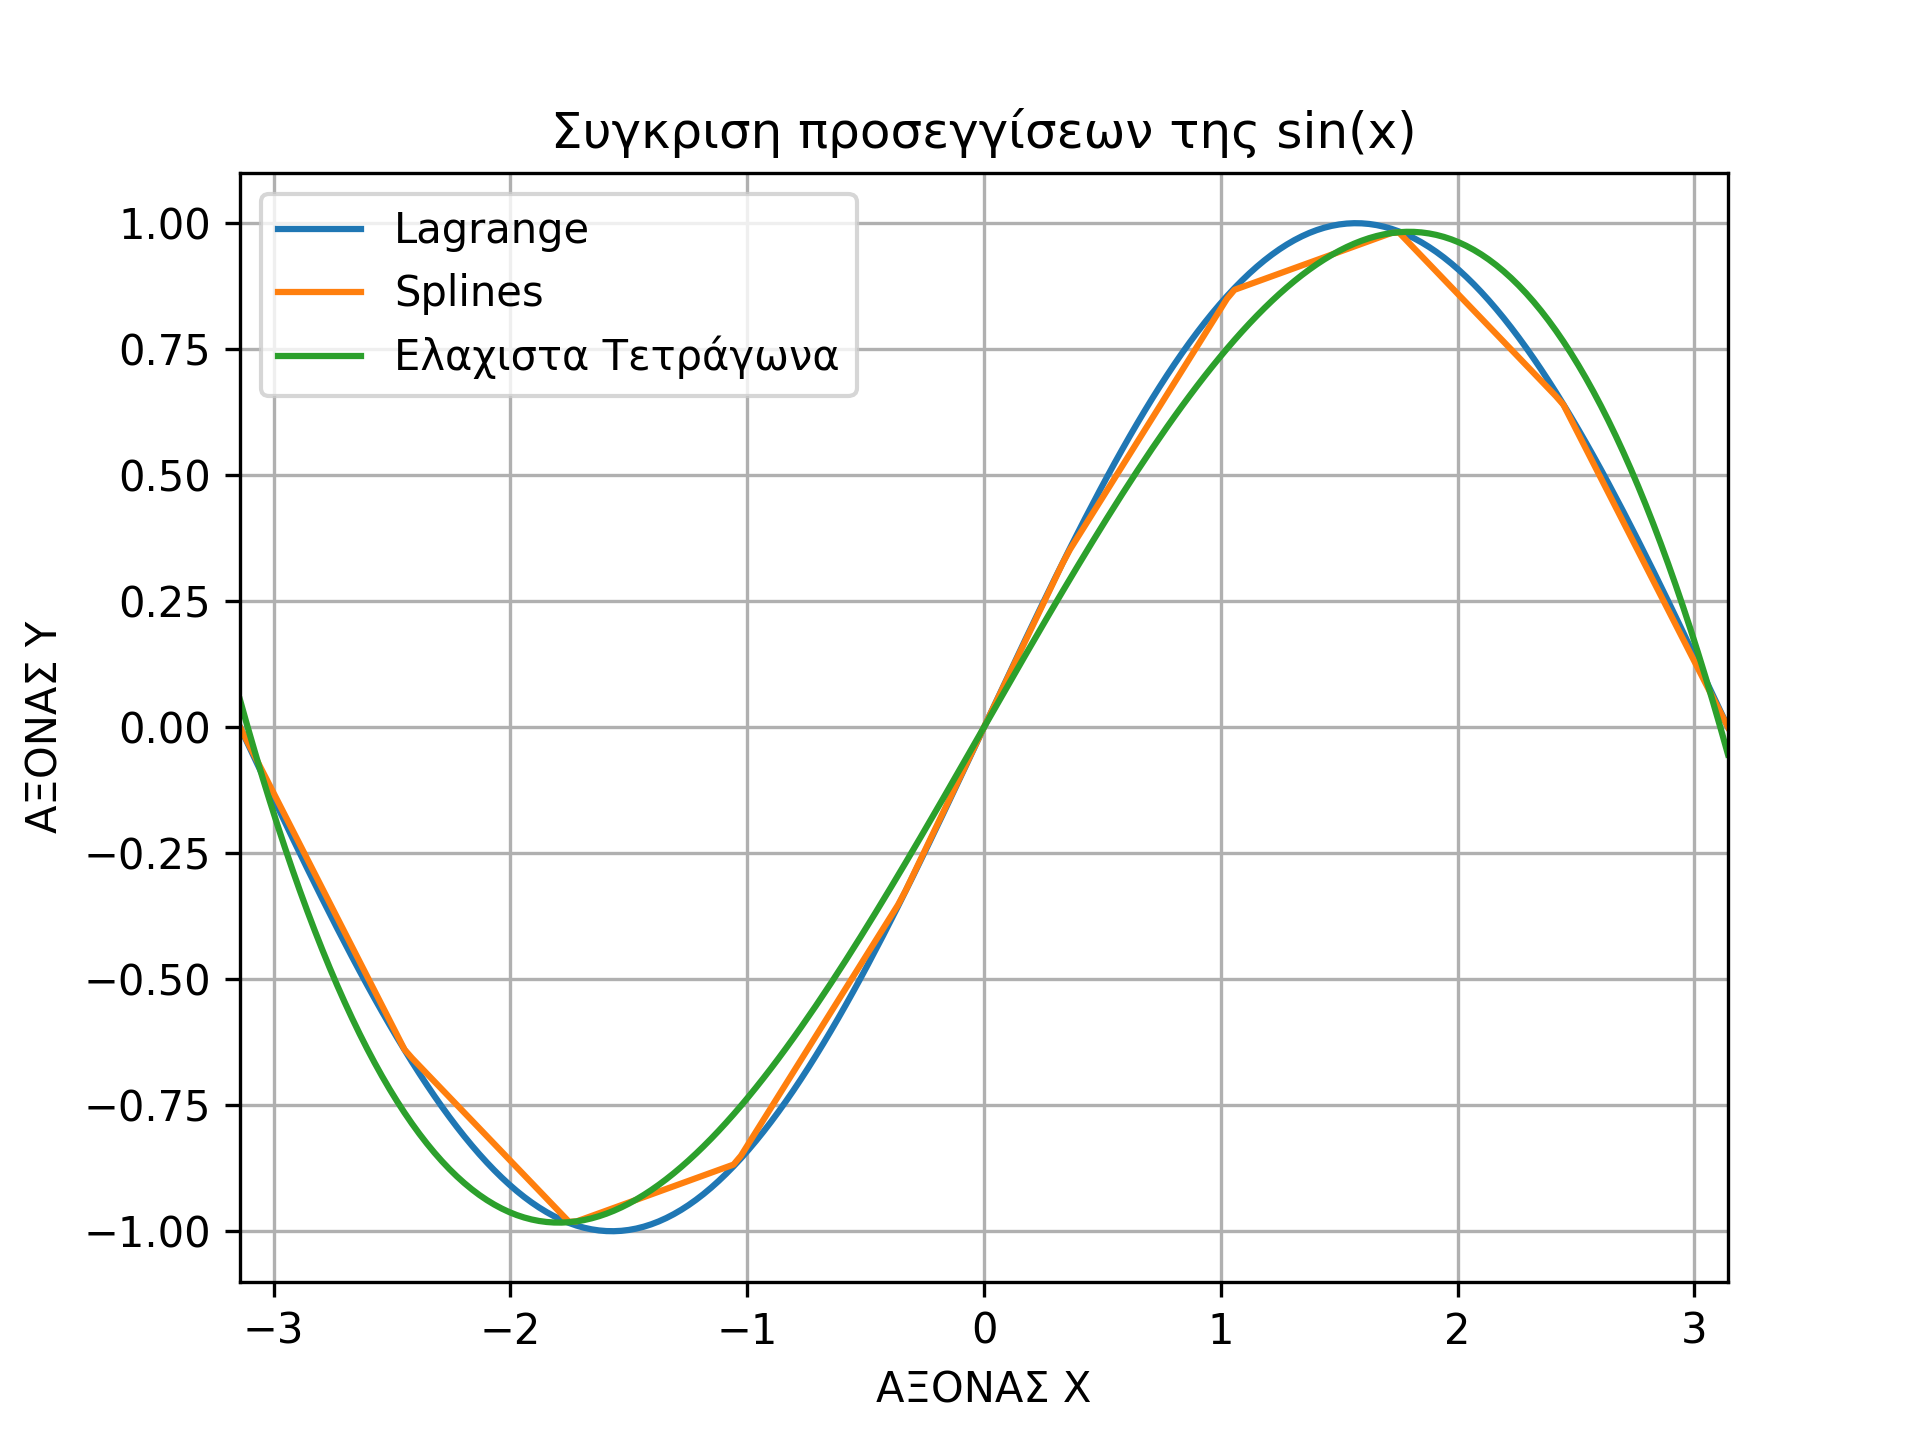
\includegraphics[width=0.8\textwidth]{graph5.png} 
\end{center} 

\newpage
\section*{Συγκρισή σφάλματος προσέγγισης}
\vspace{0.2cm}
Στη συνέχεια υπολογίζεται το σφάλμα προσέγγισης για κάθε μέθοδο σε ολα τα σημεια. Τα σφάλματα αυτα απεικονίζονται και αυτα σε ενα γραφημα, εφόσον το ζηταει η ασκηση δειχνωντας ξεκαθαρα τα διαφορετικα αποτέλεσματα που προκύπτουν απο τις μεθόδους.
\vspace{0.2cm}

\begin{center}
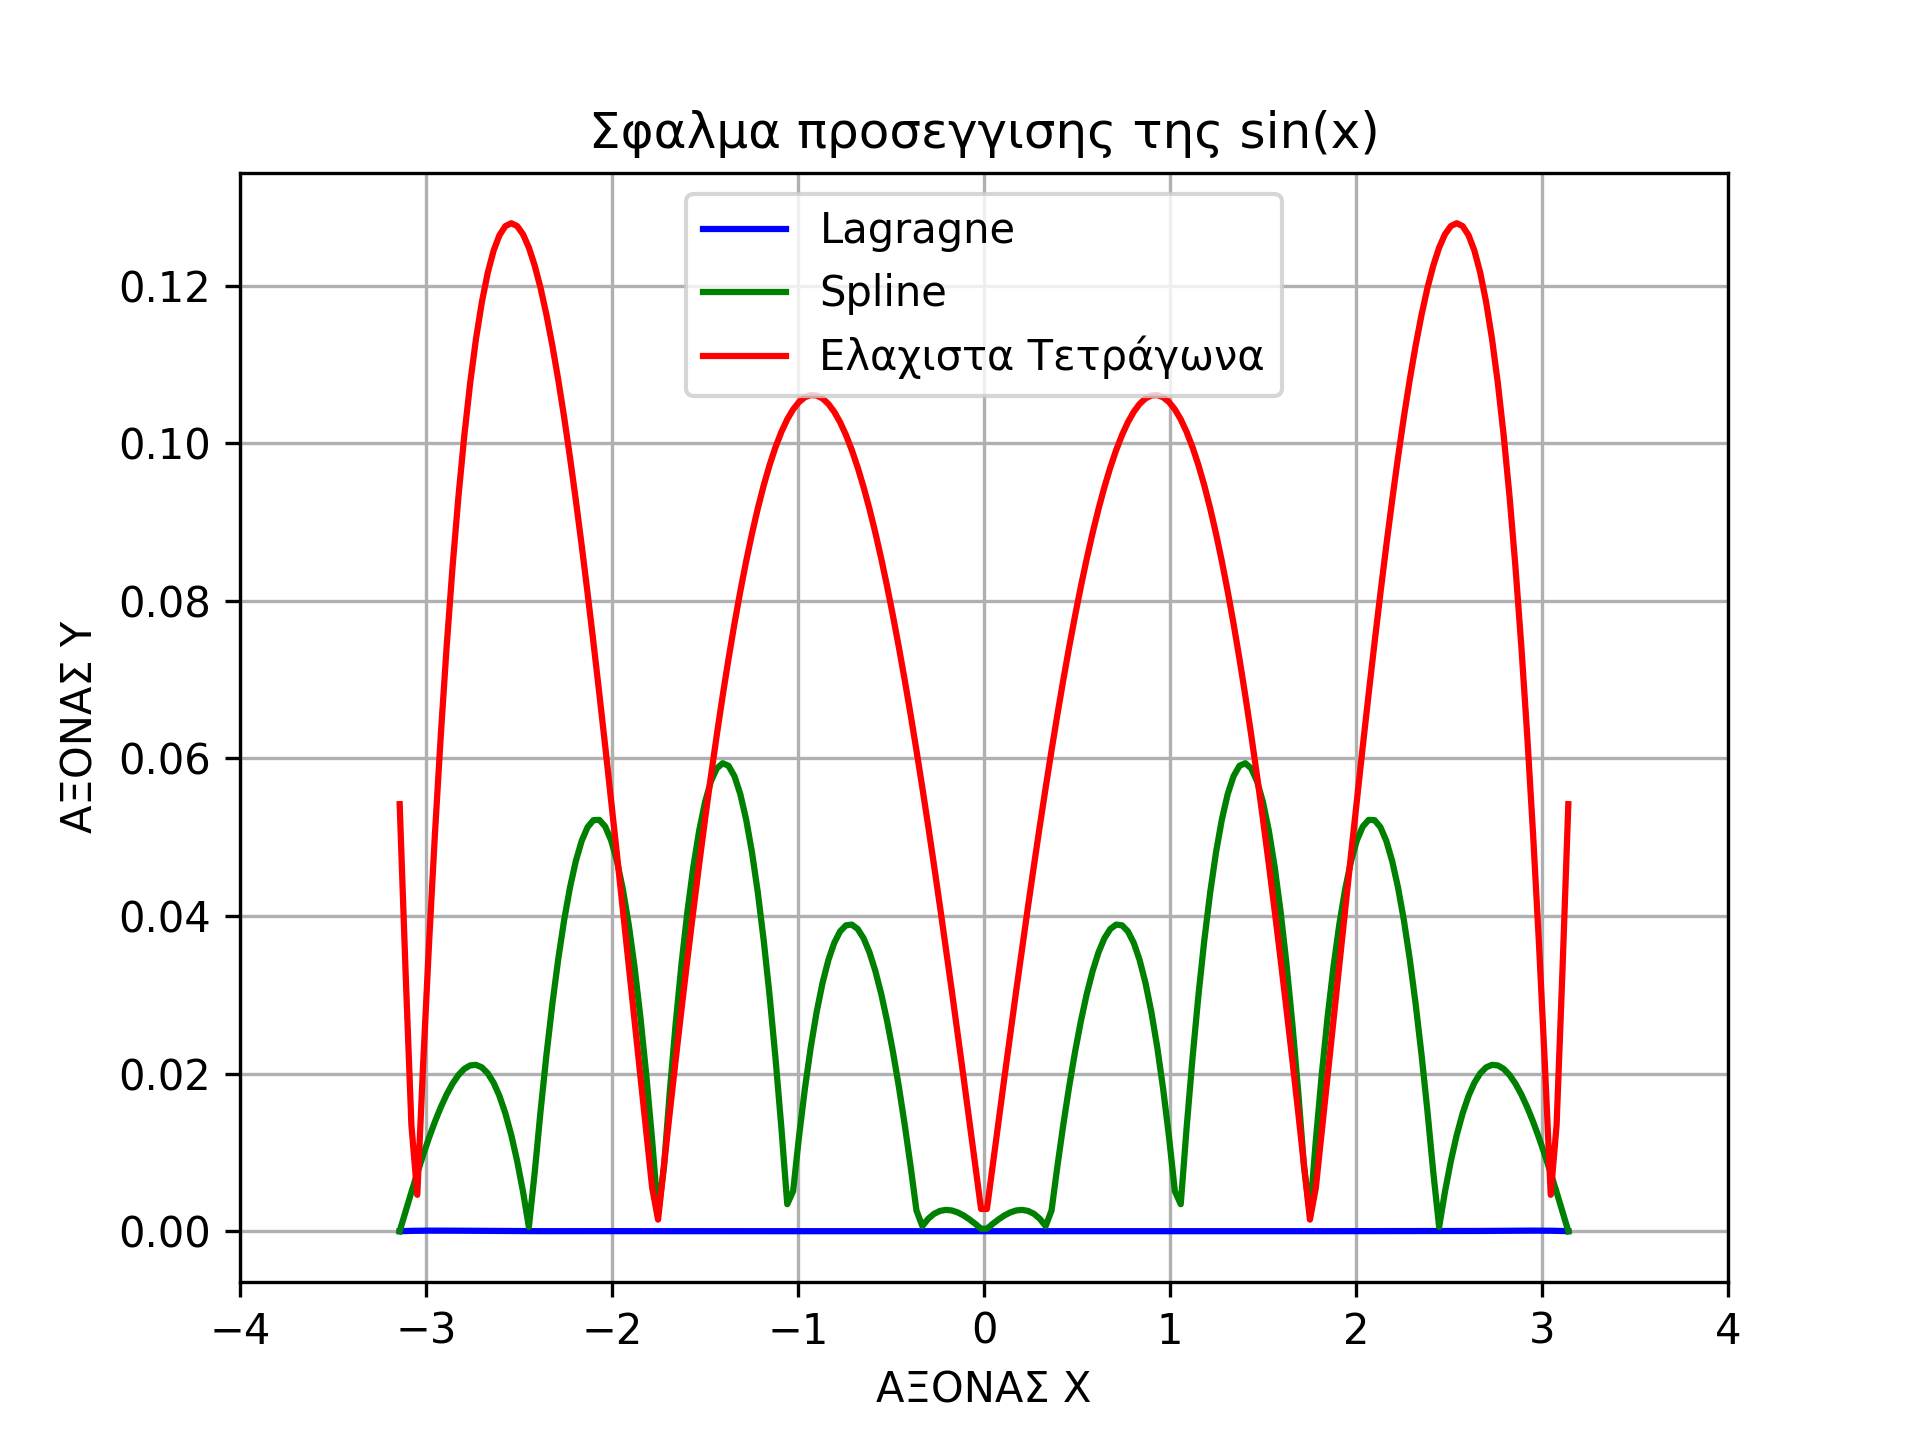
\includegraphics[width=0.8\textwidth]{graph6.png} 
\end{center} 

\vspace{0.2cm}
Απο το διάγραμμα παρατηρειται οτι η \textbf{Lagrange εμφανίζει πολυ μικρο σφάλμα}, αφου το πολυωνυμο περναει ακριβως απο τα επιλεγμένα σημεία. \textbf{Η μέθοδος των spline εμφανίζει περισσότερο σφαλμα} απο την Lagrange, αλλα η μέθοδος με το μ\textbf{εγαλυτερο σφαλμα ειναι η μέθοδος των ελαχίστων τετραγώνων}

\vspace{0.5cm}
Απο τον υπολογισμό του μέγιστου σφάλματος, προκυπτει και η παρακάτω εκτίμιση των ψηφείων ακριβείας:
\vspace{0.2cm}

\begin{itemize}
    \item \textbf{Lagrange: ψηφεια ακριβειας ≈ 4.1}
    \item \textbf{Spline: ψηφεια ακριβειας ≈ 1.2}
    \item \textbf{Ελαχιστα: Τετραγωνα ψηφεια ακριβειας ≈ 0.9}
\end{itemize}
\newpage

\section*{Ασκηση 6: μέθοδοι Simpson και Τραπεζίου}

Στην άσκηση αυτη υπολογίζεται προσεγγιστικά το ολοκλήρωμα της $\sin(x)$ στο διάστημα [0,π/2] με τη χρηση 11 σημειων και των μεθόδων \textbf{Simpson} και \textbf{τραπεζίου}. Οι μεθόδοι αυτοι υλοποιουνται στην Python.

\vspace{0.1cm}

\subsection*{Οι τύποι που χρησιμοποιηθήκαν (έχω πάρει τους τύπους απο το βιβλίο της αραν που προτείνετε)}

\vspace{0.5cm}

\begin{itemize}

\item \textbf{Κανόνας Simpson}
\[
Q_{n+1}^{S}(f) = h[\frac{1}{3}f(x_0) + 4f(x_1) + 2f(x_2) + 4f(x_3) + 2f(x_4) + ... + 4(x_{n-1}) + f(x_n)]
\]

\item \textbf{Θεωρητικό σφάλμα simpson}
\[
R_{n+1}^{S}(f) = -\frac{b-a}{180}\,h^4\,f^{(4)}(\xi)
\]

\item \textbf{Κανόνας Τραπεζίου:}
\[
Q_{n+1}^{T}(f) = h[\frac{1}{2}f(x_0) + f(x_1) + ... + f(x_{n-1}) + \frac{1}{2}f(x_n)
\]

\item \textbf{Θεωρητικό σφάλμα τραπεζίου:}
\[
R_{n+1}^{T}(f) = -\frac{b-a}{12}\, h^2\, f''(\xi)
\]

\end{itemize}

\vspace{0.5cm}

\textbf{Η ακριβης τιμή του του ολοκληρώματος ειναι ο αριθμός 1 ενω οι προσεγγίσεις των 2 μεθόδων ειναι οι εξής:}

\begin{itemize}
\item προσέγγιση \textbf{Simpson} =  1.0000033922209004
\item προσέγγιση \textbf{Tραπεζίου} = 0.9979429863543572
\end{itemize}

\vspace{0.5cm}

\textbf{Τα σφάλματα που προκύπτουν απο τις μεθόδους:}

\begin{itemize}
\item Αριθμητικό Σφάλμα \textbf{Simpson} =  3.3922209004000337e-06
\item Θεωρητικό Σφάλμα \textbf{Simpson} =  5.312841749744469e-06
\vspace{0.2cm}
\item Αριθμητικό Σφάλμα \textbf{Τραπεζίου} =  0.0020570136456428134
\item Θεωρητικό Σφάλμα \textbf{Τραπεζίου} =  0.0032298204875312307
\end{itemize}

\newpage
\section*{Ασκηση 7: Πρόβλεψη τιμών κλεισίματος}

Στην άσκηση αυτή πραγματοποείται \textbf{η πρόβλεψη της τιμης κλεισίματος} των 2 διαφορετικών μετοχών(ΕΛΙΝ, ΔΕΗ) στη μέρα των γενεθλίων μου, στις \textbf{12 Σεπτεμβριου}.

Η πρόβλεψη αυτή γίνετε με βάση τις 10 προηγούμενες τιμές κλεισίματος που ειναι διαθέσιμες.

Για την προσέγγιση αυτη θα χρησιμοποιήσουμε τη \textbf{μέθοδο ελαχίστων τετραγώνων και πολυωνυμα 2ου, 3ου, 4ου βαθμού.}

Η υλοποίηση της μεθόδου ελαχίστων τετραγώνων έχει υλοποιηθεί στην python όπως και σε προηγουμένη άσκηση.

\vspace{0.5cm}

\subsection*{Συγκρισή πολυωνύμων}

Για κάθε μετοχή υπολόγισα το \textbf{μέγιστο απόλυτο σφάλμα} με βάση τις 10 τιμές που είχα.

\vspace{0.5cm}

Για τη \textbf{1η Μετοχή} τα \textbf{σφάλματα} που προέκυψαν είναι:

\begin{itemize}
\item 2ου βαθμού: 0.0498
\item 3ου βαθμού: 0.0492  
\item 4ου βαθμου: 0.0481
\end{itemize}

\vspace{0.2cm}

Για τη \textbf{2η Μετοχή} τα \textbf{σφάλματα} που προέκυψαν είναι:

\begin{itemize}
\item 2ου βαθμου:  0.2065
\item 3ου βαθμου:  0.2114
\item 4ου βαθμου:  0.1795
\end{itemize}

\vspace{0.2cm}
Παρατηρούμε οτι το πολυώνυμο 4ου βαθμού έχει το μικρότερο σφάλμα
\vspace{0.5cm}

\newpage
\subsection*{Πρόβλεψη τιμής κλεισίματος στις 12 Σεπτεμβρίου}

\vspace{0.2cm}

Για τη \textbf{1η Μετοχή οι προβλέψεις} που προέκυψαν είναι:

\begin{itemize}
    \item 2ου βαθμού: 2.5791
    \item 3ου βαθμού: 2.5733
    \item 4ου βαθμού: 2.5808
    \item Ενω η \textbf{πραγματική τιμή κλεισίματος είναι} 2.5600
\end{itemize}

\vspace{0.5cm}

Για τη \textbf{2η Μετοχή οι προβλέψεις} που προέκυψαν είναι:
\begin{itemize}
    \item 2ου βαθμού: 14.2901
    \item 3ου βαθμού: 14.3403
    \item 4ου βαθμού: 15.0808
    \item Ενω η πραγματικη τιμή κλεισίματος ειναι 14.3500
\end{itemize}

\vspace{0.5cm}

Οι \textbf{τιμές} που προκυπτουν \textbf{ειναι πολύ κοντινές στην πραγματική τιμή κλεισίματος}, άρα οι μεθόδοι μας δουλευούν σωστά.

\newpage
\subsection*{Πρόβλεψη για τις επόμενες 5 τιμές κλεισίματος}

Θα χρησιμοποιήσω το πολυώνυμο του 2ου βαθμού για την πρόβλεψη των επόμενων 5 τιμών.

\vspace{0.5cm}

Για τη \textbf{1η Μετοχή} οι \textbf{επόμενες 5 προβλέψεις} είναι:

\begin{itemize}
    \item η 11η =  2.6205
    \item η 12η =  2.6681
    \item η 13η =  2.7221
    \item η 14η =  2.7823
    \item η 15η =  2.8488
\end{itemize}

\vspace{0.5cm}


Για τη \textbf{2η Μετοχή} οι \textbf{επόμενες 5 προβλέψεις} είναι:

\begin{itemize}
    \item η 11η =  14.3440
    \item η 12η =  14.4029
    \item η 13η =  14.4666
    \item η 14η =  14.5353
    \item η 15η =  14.6089
\end{itemize}

Οι προβλέψεις που προκύπτουν \textbf{παρουσιάζουν μια σταδιακή αύξηση} η οποία ενα περίπου \textbf{συμφωνέι} με τις \textbf{πραγματικές τιμές κλεισίματος}, αρα είναι \textbf{ρεαλιστικές}.
\end{document}



